
%==============================================================================
%== template for LATEX poster =================================================
%==============================================================================
%
%--A0 beamer slide-------------------------------------------------------------
\documentclass[final]{beamer} % use beamer
\usepackage[orientation=portrait,
            size=a0,          % poster size
            scale=1.3        % font scale factor
           ]{beamerposter}    % beamer in poster size
%
%--some needed packages--------------------------------------------------------

\usepackage[utf8]{inputenc}
\usepackage[T1]{fontenc}
\usepackage[portuguese]{babel}

\usepackage{lipsum}
%
%==The poster style============================================================
\usetheme{cpbgposter}            % our poster style
%--set colors for blocks (without frame)---------------------------------------
  \setbeamercolor{block title}{fg=ngreen,bg=white}
  \setbeamercolor{block body}{fg=black,bg=white}
%--set colors for alerted blocks (with frame)----------------------------------
%--textcolor = fg, backgroundcolor = bg, dblue is the jacobs blue
  \setbeamercolor{block alerted title}{fg=white,bg=dblue!70}%frame color
  \setbeamercolor{block alerted body}{fg=black,bg=dblue!10}%body color
%
%==Titel, date and authors of the poster=======================================
\title[]{Estruturação do Site da Biblioteca de Processamento de Imagens Biomédicas (BIAL)}
\author[Lucas Lellis]{Lucas Santana Lellis \and Prof. Dr. Fábio Augusto Menocci Cappabianco}
\institute[ICT - UNIFESP]{Instituto de Ciência e Tecnologia, Universidade Federal de São Paulo}
\date{São José dos Campos - SP}
%
%==some usefull qm commands====================================================
%  |x>
\newcommand{\ket}[1]{\left\vert#1\right\rangle}
%  <x|
\newcommand{\bra}[1]{\left\langle#1\right\vert}
%  <x|y>
\newcommand{\braket}[2]{\left< #1 \vphantom{#2}\,
                        \right\vert\left.\!\vphantom{#1} #2 \right>}
%  <x|a|y>
\newcommand{\sandwich}[3]{\left< #1 \vphantom{#2 #3} \right|
                          #2 \left|\vphantom{#1 #2} #3 \right>}
%  d/dt
\newcommand{\ddt}{\frac{d}{dt}}
%  D/Dx
\newcommand{\pdd}[1]{\frac{\partial}{\partial#1}}
%  |x|
\newcommand{\abs}[1]{\left\vert#1\right\vert}
%  k_{x}
\newcommand{\kv}[1]{\mathbf{k}_{#1}}
%==============================================================================
%==the poster content==========================================================
%==============================================================================
\begin{document}
%--the poster is one beamer frame, so we have to start with:
\begin{frame}[t]
%--to seperate the poster in columns we can use the columns environment
 \begin{columns}[t] % the [t] options aligns the columns content at the top
%--the left column-------------------------------------------------------------
  \begin{column}{0.28\paperwidth}% the right size for a 3-column layout
%--abstract block--------------------------------------------------------------
   \begin{alertblock}{Resumo}
	   Com o objetivo de promover a divulgação do Grupo de Inovação Baseada em Imagens e Sinais (GIBIS), e seus projetos chave, como a Biomedical Image Analysis Library (BIAL), foi desenvolvida uma página na web sob o domínio \textbf{hhtp://gibis.unifesp.br}.
	   
	   Baseada na Rails framework, o website possui suporte ao cadastro de usuários,
	   que podem alterar seus perfis no sistema, com foto, breve resumo, e informações de contato.
   \end{alertblock}
   \vskip2ex
%--requirements block-----------------------------------------------------------
   \begin{block}{Introdução}
   		O \textbf{Grupo de Inovação Baseada em Imagens e Sinais} foi formado em 2012 pelos docentes Fábio Augusto Menocci Cappabianco e Jaime Shinsuke Ide, e conta com a participação de 10 docentes e alunos dos cursos de Bacharelado em Ciência e Tecnologia, Engenharia Biomédica, Bacharelado e Mestrado em Ciência da Computação.
   		
   		Este grupo tem desenvolvido diversos trabalhos na área de processamento e análise de imagens e sinais biomédicos, publicando seus resultados em periódicos e conferências nacionais e internacionais de renome.
 
   		Um dos trabalhos mais significativos é uma biblioteca para processamento de imagens médicas denominada \textbf{Biomedical Image Analysis Library}, que realiza operações sobre diversas modalidades de imagens, como Tomografia Computadorizada e Ressonância Magnética. A figura \ref{fig:bial} possui uma captura de tela da interface gráfica da BIAL.
   		
   		\begin{figure}[ht]
   			\begin{center}
   				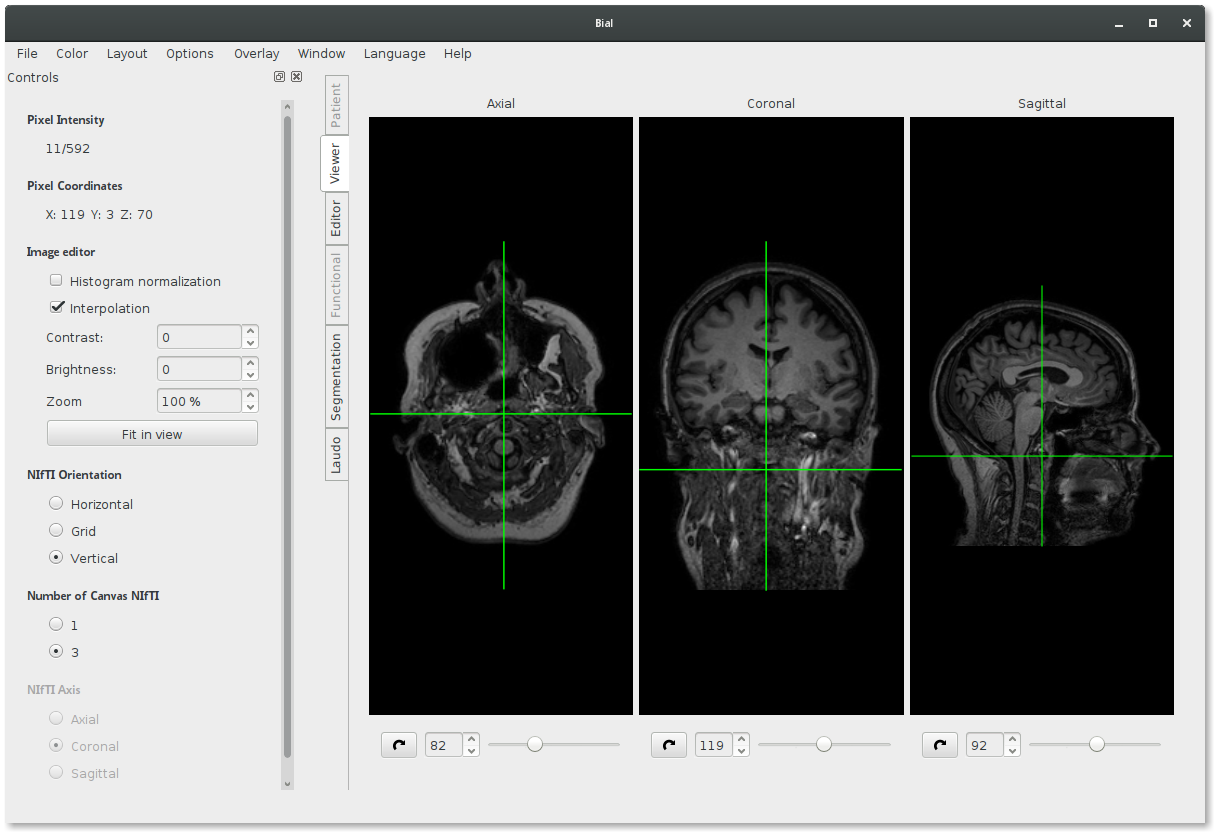
\includegraphics[width=1.0\textwidth]{./figures/bial}
   				\caption{Captura de tela da interface da BIAL \label{fig:bial}}
   				%  And a throught view of a female of the species with its sheath visible.}
   			\end{center}
   		\end{figure}
   		
   		
   		Agora com um laboratório equipado, e um número considerável de colaboradores, chega o momento de aumentar a divulgação do grupo. Assim o projeto tem como objetivo disponibilizar um \textbf{site na internet}, assim como a documentação e distribuição da BIAL para o uso da comunidade científica.
   \end{block}
   \vskip2ex
%--features block---------------------------------------------------------------
   \begin{block}{Objetivos}
	Com o intuito de promover a divulgação do grupo e seus projetos e contribuições para a comunidade científica, o projeto tem como objetivos:
    \vskip1ex
    \begin{itemize}
     \item {\bf Desenvolvimento da identidade visual do Grupo e da Bial}\\
		O desenvolvimento dos logotipos do GIBIS, e da BIAL, assim como o front-end do website são marcas importantes que definem uma identidade, que será mantida, e conhecida por muito tempo.
     \item {\bf Disponibilização de informações sobre projetos e pesquisadores.}\\
	     O website deve conter um breve resumo, assim como informações de contato sobre os diversos pesquisadores do grupo, assim como seus projetos e agências de fomento.
    \end{itemize}
   \end{block}
   \vskip1ex

  \end{column}
%===rightcolumn=================================================================
% here the the middle and right column are put into one big column, this allows
% to change between 2 and 3 column style
  \begin{column}{0.60\paperwidth} %thats the big right column
%--Examples block---------------------------------------------------------------
	\begin{block}{Metodologia}
		Tendo como objetivo o aprendizado de forma gradual e produtiva, o projeto foi desenvolvido em diferentes etapas:
		\begin{columns}[t,totalwidth=0.60\paperwidth]
			\begin{column}{0.28\paperwidth}
			\begin{itemize}
		    	\item {\bf Estudo sobre princípios de HTML e CSS}\\
					Html e CSS são a base do front-end da web, sendo os responsáveis por definir a forma em que a página é exibida no browser.
				\item {\bf Desenvolvimento da interface}\\
					Foi feita uma versão inicial do front-end do website utilizando a tecnologia \textbf{Bootstrap}.
					
					Bootstrap é um conjunto de componentes de interface que facilita a criação de websites responsivos e compatíveis com dispositivos móveis.
			\end{itemize}
			\end{column}
			\begin{column}{0.28\paperwidth}
				\begin{itemize}
					\item {\bf Elaboração da identidade visual}\\
						Foram utilizadas tecnologias livres para o desenvolvimento da identidade visual, como o \textbf{Gimp} e \textbf{Inkscape}, poderosas ferramentas de edição de imagem.
					\item {\bf Implementação das funcionalidades}\\
						Baseando-se na interface desenvolvida, e com o auxílio da tecnologia \textbf{Ruby on Rails}, é possível implementar funcionalidades dinâmicas, integradas ao banco de dados \textbf{MySql}.
				\end{itemize}
			\end{column}
		\end{columns}
		   		
   		\begin{figure}[ht]
   			\begin{center}
   				
\includegraphics[width=1.0\textwidth]{./figures/tecnologias}
   				\caption{Tecnologias utilizadas no projeto, da esquerda para a direita: Html5, Css3, Bootstrap, Gimp, Inkscape, Ruby on Rails, e Mysql \label{fig:tecnologias}}
   				%  And a throught view of a female of the species with its sheath visible.}
   			\end{center}
   		\end{figure}
		   		
		Na figura \ref{fig:tecnologias} estão representadas as diferentes tecnologias utilizadas durante todo o processo.
	\end{block}
	\begin{block}{Resultados e discussão}
	   	Após meses de desenvolvimento, é possível exibir diferentes resultados e funcionalidades interessantes, como:
		\begin{columns}[t,totalwidth=0.60\paperwidth]
			\begin{column}{0.28\paperwidth}
				\begin{itemize}
					\item {\bf Identidade visual}\\
			   		\begin{figure}[ht]
			   			\begin{center}
			   				
\includegraphics[width=0.65\textwidth]{./figures/identidade}
			   				\caption{Logotipos desenvolvidos. Em ordem: Logo do Gibis, Logo da BIAL, e ícone da BIAL. \label{fig:identidade}}
			   			\end{center}
			   		\end{figure}
			   		A figura \ref{fig:identidade} mostra a id. visual desenvolvida para o gibis, e BIAL.
					%--------- Home Page  --------------- %
					\item {\bf Home page}\\
					\begin{figure}[ht]
						\begin{center}
							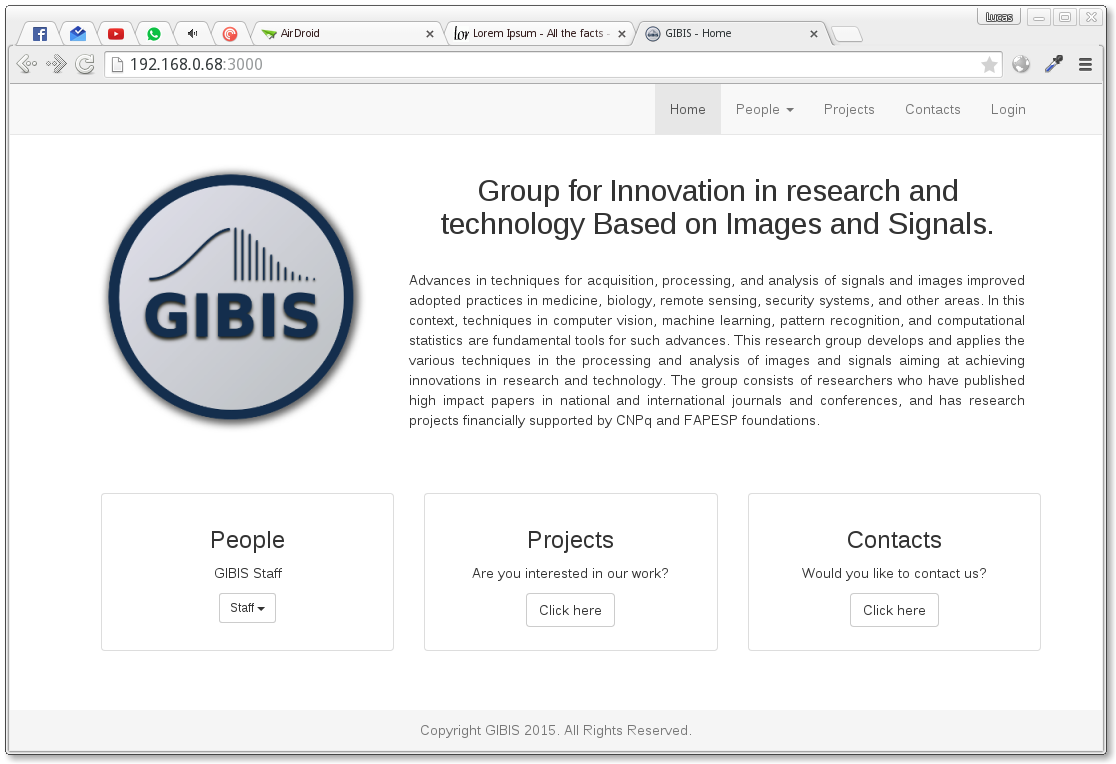
\includegraphics[width=0.65\textwidth]{./figures/home}
							\caption{Imagens da home page. \label{fig:home}}
						\end{center}
					\end{figure}
					Foi implementada a home page do grupo, conforme a figura \ref{fig:home}.
					%--------- Projetos  --------------- %
					\item {\bf Página da Bial}\\
					\begin{figure}[ht]
						\begin{center}
							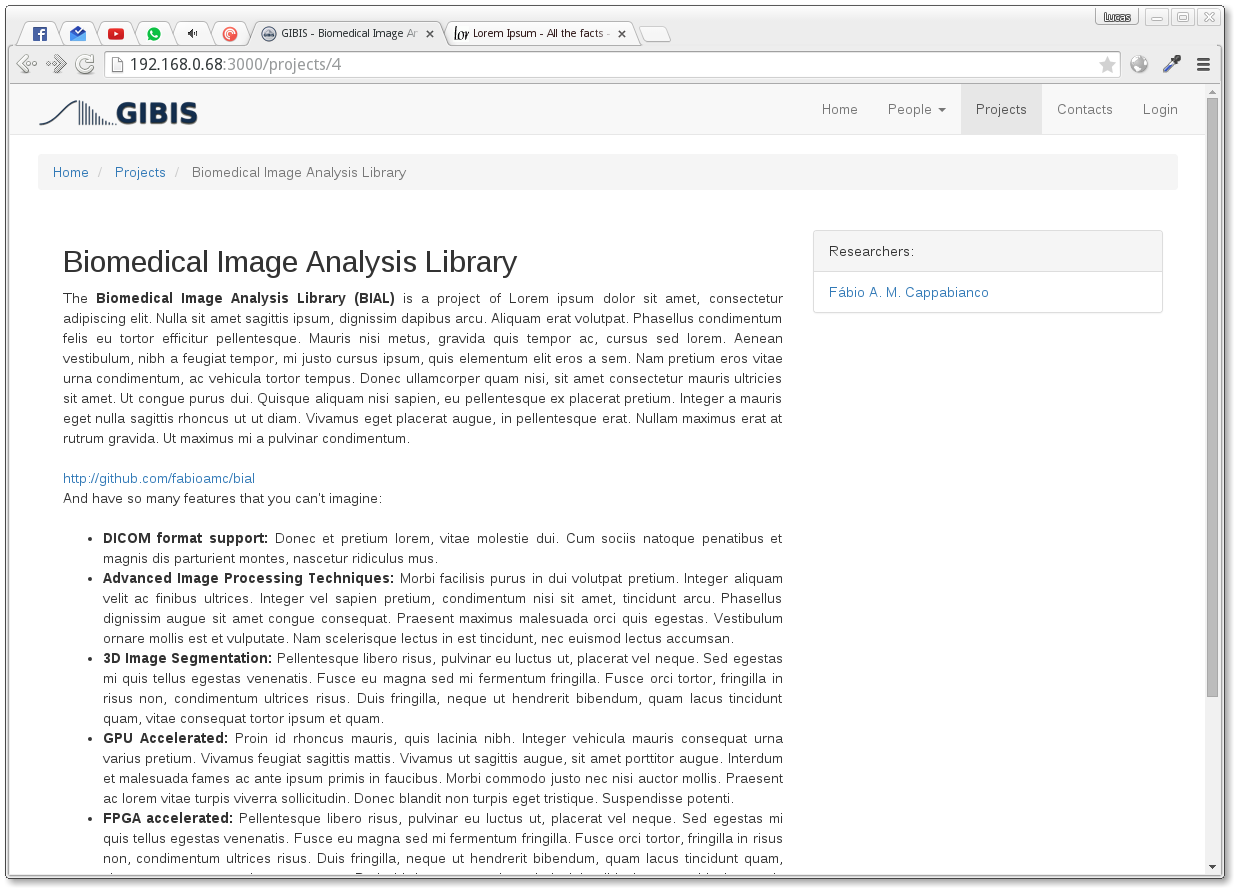
\includegraphics[width=0.65\textwidth]{./figures/project}
							\caption{Página do projeto BIAL. \label{fig:projeto}}
						\end{center}
					\end{figure}
					Dentro do website, existe uma página dedicada à BIAL ( figura \ref{fig:projeto} ).
					
				\end{itemize}
			\end{column}
			\begin{column}{0.28\paperwidth}
				\begin{itemize}
					\item {\bf Funcionalidades dinâmicas}\\
					\begin{figure}[ht]
						\begin{center}
							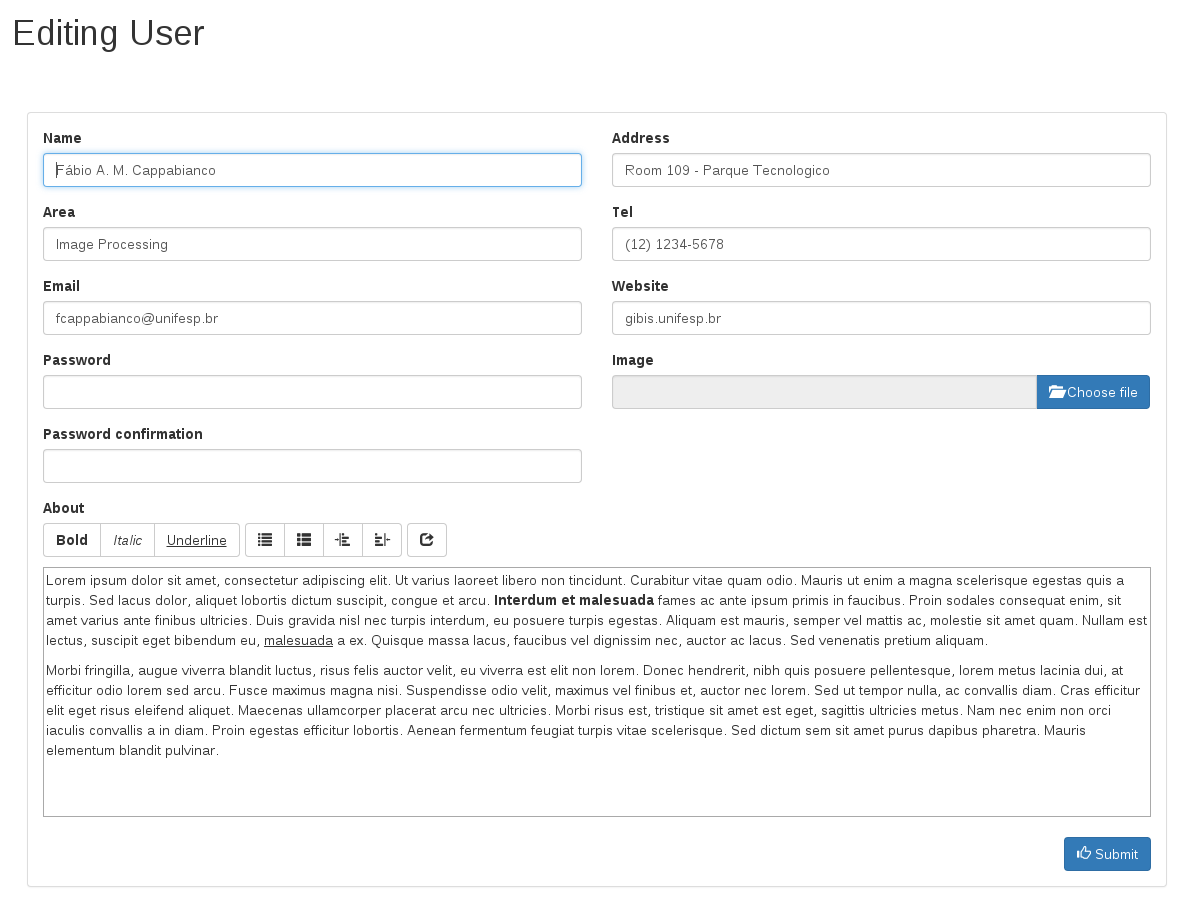
\includegraphics[width=0.75\textwidth]{./figures/edicao}
							\caption{Interface de edição. \label{fig:edicao}}
						\end{center}
					\end{figure}
					Foram desenvolvidas funcionalidades de edição de usuários, projetos e patrocinadores, além das funcionalidades de login, perfil administrador, recuperação de senha e ativação de contas. A figura \ref{fig:edicao} mostra a interface de edição de perfil de usuário.
					\item {\bf Interface móvel}\\
					\begin{figure}[ht]
						\begin{center}
							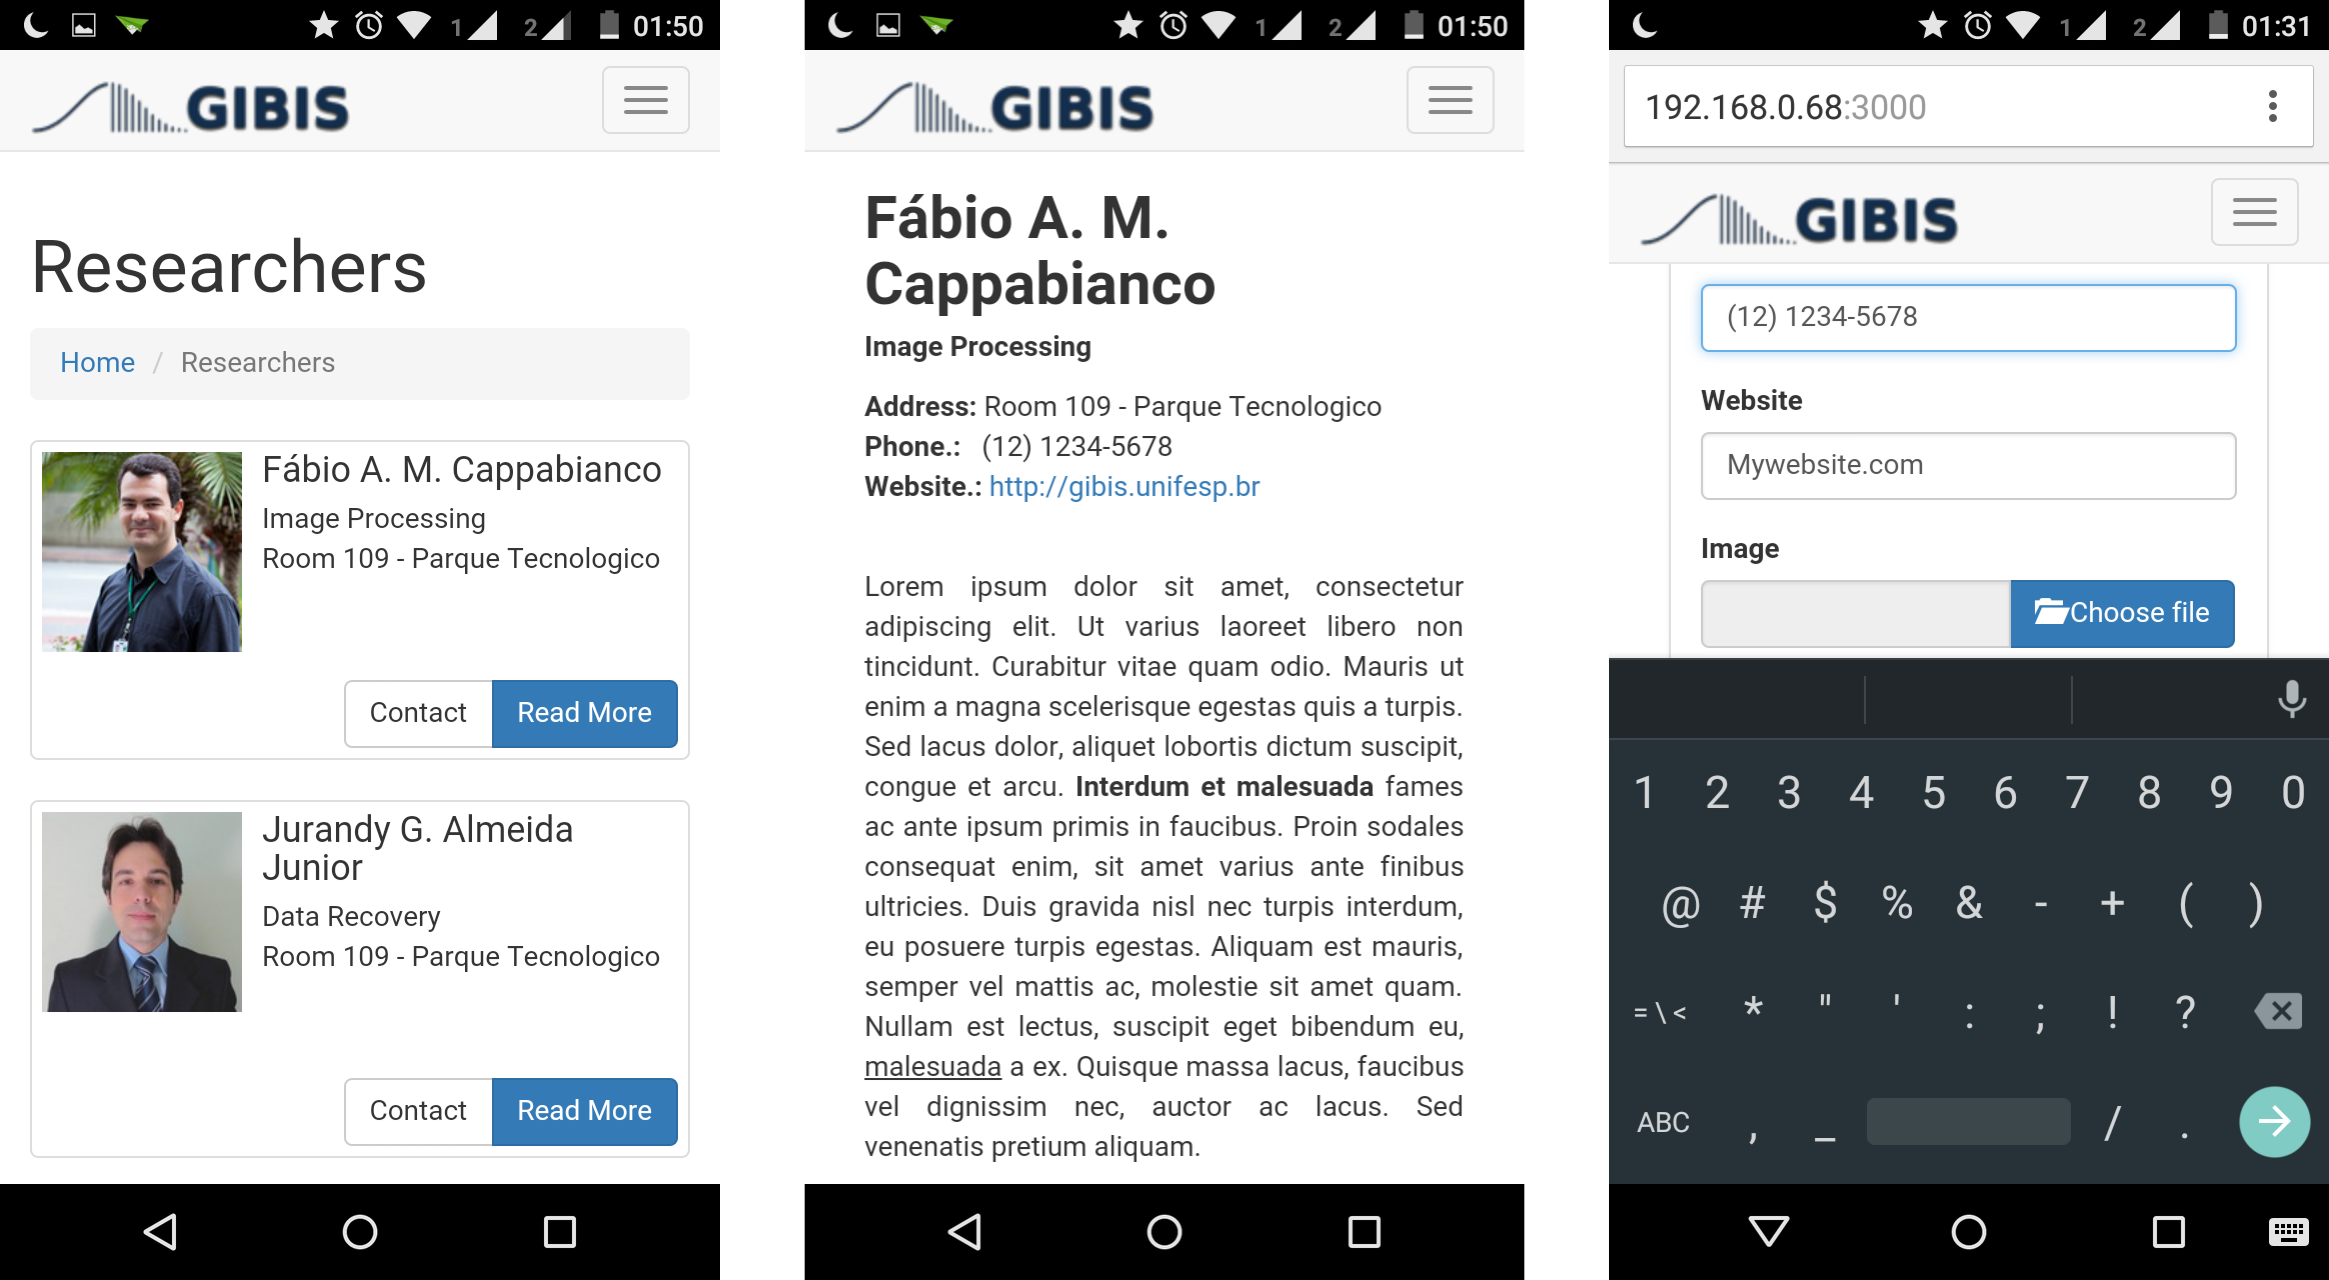
\includegraphics[width=1.0\textwidth]{./figures/mobile}
							\caption{Imagem da interface móvel. \label{fig:mobile}}
						\end{center}
					\end{figure}
					Um dos destaques é a utilização do Bootstrap para a construção da interface responsiva, que se adapta à dispositiveis móveis (figura \ref{fig:mobile}).
					
				\end{itemize}
			\end{column}
		\end{columns}
	\end{block}
		\begin{columns}[t,totalwidth=0.60\paperwidth]
			\begin{column}{0.38\paperwidth}
				\begin{block}{Conclusões}
					A princípio o site seria composto de páginas estáticas, porém, a tecnologia escolhida proporcionou com alta qualidade, diversas funcionalidades dinâmicas, como a edição das páginas de projetos e pesquisadores, assim como o suporte ao cadastro de usuários.
					
					O projeto proporcionou importantes oportunidades de aprendizado na área de desenvolvimento web, design gráfico, engenharia de software, e banco de dados. Sendo uma ótima oportunidade de assimilar novas tecnologias ao currículo, como o Bootstrap, e o Ruby on Rails.		
				\end{block}
			\end{column}
			\begin{column}{0.18\paperwidth}
				\newline
				\newline
				\begin{alertblock}{Agradecimentos}
					Agradecemos ao Programa de Bolsas de Iniciação à Gestão, e à Universidade Federal de São Paulo por tornarem este projeto possível.
				\end{alertblock}
			\end{column}
		\end{columns}

   \end{column}
 \end{columns}
\end{frame}
\end{document}
